\chapter{GPS and Monte Carlo Localization}
\label{chap:gps_and_mcl}

This chapter discusses two approaches to using GPS receiver as a correction input
to Monte Carlo localization. One based on pseudorange measurements and one based on
WGS84 pre-calculated data.



\section{Position Domain Integration}
Position domain integration means combining the calculated position and velocity from
GPS with other sensors.

Most GPS receivers 

This approach has the advantage of being very simple 

\begin{itemize}
\item Using complete fixes from receiver
\item Simple, less CPU intensive
\end{itemize}

\subsection{Sensor Model}
\label{sec:wgs84_hdop_error}

\begin{figure}[htp]
	\centering
	\noindent\makebox[\textwidth]{
	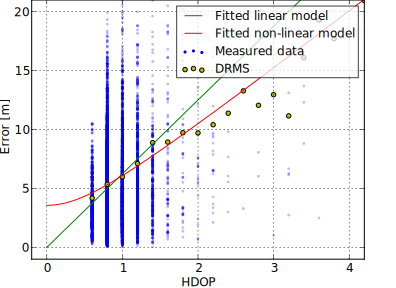
\includegraphics{plots/wgs84_hdop_error.pdf}
	}
	\caption{Measurement errors vs. HDOP.}
	\label{fig:wgs84_hdop_error}

	% cube@duskwalker ~/diplomka/impl $ ./wgs84_errors.py --no-show --plotted-sample-count 10000 --max-plot-hdop 4 --max-plot-error 20 --save-hdop-plot ../text/img/wgs84_hdop_error.svg recordings/processed_numpy_arrays/month_wgs84.npy 
	% /usr/lib/python2.7/site-packages/mpl_toolkits/__init__.py:2: UserWarning: Module argparse was already imported from /usr/lib/python2.7/argparse.pyc, but /usr/lib/python2.7/site-packages is being added to sys.path
	%   __import__('pkg_resources').declare_namespace(__name__)
	% 2012-10-07 23:51:44,958 - root - INFO - Done. Have 2363458 fixes
	% 2012-10-07 23:51:44,958 - root - INFO - Projecting
	% 2012-10-07 23:51:45,803 - root - INFO - Done
	% 2012-10-07 23:51:45,804 - root - INFO - Calculating distances
	% 2012-10-07 23:51:46,090 - root - INFO - Done
	% 2012-10-07 23:51:46,090 - root - INFO - HDOP statistics
	% Fitted linear model: 6.25518909128 * HDOP
	% Fitted non linear model: sqrt((4.94140672924 * HDOP)**2 + 3.5682895544**2)
	% 2012-10-07 23:51:52,734 - root - INFO - Done
	% Scatter plots will only use 1/236 samples
	% 99.66% is in the area 4.0x20.0
	% 2012-10-07 23:52:59,803 - root - INFO - Saved ../text/img/wgs84_hdop_error.svg

\end{figure}

For modelling the error we basically follow \cite{www-wilson}.

Horizontal component of the position error  \(\vect{\delta R}\) is modelled using Rayleigh distribution
parameterized with HDOP of the measurement:
\begin{equation}
	\Prob(\norm{\vect{\delta R}} < x \mid \HDOP) =
		1 - e^{-x^2/2\sigma(\HDOP)^2}
\end{equation}

Parameter \(\sigma(\HDOP)\) of the distribution is chosen to fit the DRMS values using a maximum likehood estimate
\begin{equation}
	\sigma = \frac{\mathrm{DRMS}}{\sqrt{2}}
\end{equation}

\autoref{fig:wgs84_hdop_error} plots position error versus HDOP value.
Blue dots represent the measured data, yellow dots the DRMS values.
Green line is the fitted theoretical linear model
\begin{equation}
\mathrm{DRMS}(\HDOP) = \num{6.255} \HDOP
\end{equation}
and red curve is the fitted non linear model from \cite{www-wilson}
\begin{equation}
\mathrm{DRMS}(\HDOP) = \sqrt{(\num{4.941}\HDOP)^2 + \num{3.568}^2}
\end{equation}
Both of these models were fitted to the data using least squares weighted with counts of samples
for each HDOP.

Limited resolution of the HDOP values in input data is visible in the plot,
another interesting fact is, that only relatively low HDOP values were encountered.
This can be seen in \autoref{fig:hdop_hist}.

A problem that is hard to avoid with this approach is that position errors of the
receiver output are correlated.
This is in part because errors of the individual satellite measurements are correlated
(which is discussed in \ref{sec:measurement_domain_correlation}), but another major reason
is the \enquote{inertia} added by the Kalman filter.
This kind of correlation obviously breaks the independence assumptions of Markov
localization defined in \ref{sec:markov_assumptions}, but in this case we chose to ignore
the problem. \todo{Or not.}

\section{Measurement Domain Integration}
\label{sec:measurement_domain}

\begin{itemize}
\item Using each pseudorange measurement
\item Maybe better localization, no assumptions about vehicle properties
\end{itemize}

\subsection{Static Environment Assumption}
\label{sec:gps-mcl-static-env}
Monte Carlo Localization assumes that the environment is static, but we need to
localize according to moving satellites.
To avoid this problem we will hide satellite motion into the robot state and sensor model.

\subsection{Error distribution}
Normal distribution (???)

\subsubsection{Error correlation}
\label{sec:measurement_domain_correlation}
Keep atmospheric delays as part of the localization state?

\subsection{Preprocessing}
\begin{itemize}
\item ???
\end{itemize}

\subsection{Initial estimate}
\begin{itemize}
\item starting as position domain, later switching to measurement domain
\end{itemize}

\subsection{Simplifications}
\begin{itemize}
\item Ignoring altitude (???)
\item Additional 1D kalman for altitude (???)
\item Additional 1D kalman for receiver clock error (???)
\end{itemize}
